%==============================================================================
% Chapitre 58 - Les gerbes de grenaille
%==============================================================================

\section{Introduction}

Lorsqu'une cartouche à grenaille est tirée, les projectiles quittent le canon
sous la forme d'un ensemble compact qui se disperse progressivement.

L'ensemble des impacts obtenus sur une cible est appelé :

\begin{quote}
gerbe
\end{quote}

L'étude de cette gerbe constitue un élément fondamental de la balistique des
fusils de chasse.

\begin{aretenir}

La qualité d'une cartouche à grenaille s'évalue principalement par l'analyse
de la gerbe obtenue sur cible.

\end{aretenir}

\section{Formation de la gerbe}

À la sortie du canon, les projectiles sont encore très proches les uns des
autres.

Au cours du vol, ils s'écartent progressivement sous l'effet de plusieurs
phénomènes :

\begin{itemize}
    \item différences de vitesse ;
    \item collisions entre projectiles ;
    \item perturbations aérodynamiques ;
    \item influence du choke ;
    \item influence de la bourre.
\end{itemize}

\section{Dispersion naturelle}

Même en l'absence de choke, la grenaille ne reste pas regroupée.

Une dispersion progressive apparaît naturellement dès la sortie du canon.

\section{Évolution avec la distance}

Lorsque la distance augmente :

\begin{itemize}
    \item le diamètre de la gerbe augmente ;
    \item la densité des impacts diminue ;
    \item les espaces entre projectiles deviennent plus importants.
\end{itemize}

\begin{figure}[htbp]
\centering

\begin{tikzpicture}[scale=1]

% Canon
\draw[thick] (0,2) rectangle (1,3);

\node[left] at (0,2.5)
{Canon};

% Gerbes
\draw[dashed] (1,2.5) -- (4,3);
\draw[dashed] (1,2.5) -- (4,2);

\draw[dashed] (1,2.5) -- (7,3.8);
\draw[dashed] (1,2.5) -- (7,1.2);

\draw[dashed] (1,2.5) -- (10,4.8);
\draw[dashed] (1,2.5) -- (10,0.2);

% Sections
\draw (4,2) -- (4,3);
\draw (7,1.2) -- (7,3.8);
\draw (10,0.2) -- (10,4.8);

\node[below] at (4,1.7) {Courte};
\node[below] at (7,0.9) {Moyenne};
\node[below] at (10,-0.1) {Longue};

\end{tikzpicture}

\caption{La gerbe s'élargit progressivement avec la distance.}
\label{fig:evolution_gerbe_distance}

\end{figure}

\section{Pourquoi la densité est importante}

La présence d'impacts sur la cible ne suffit pas.

Une densité insuffisante peut réduire l'efficacité du tir.

L'objectif est généralement d'obtenir une couverture suffisamment homogène.

\begin{figure}[htbp]
\centering

\begin{tikzpicture}

% Dense
\draw (0,0) circle (2);

\foreach \x/\y in {
-1.3/0.8,-1.0/0.2,-1.1/-0.7,
-0.5/1.1,-0.4/0.4,-0.4/-0.3,-0.5/-1.0,
0.3/1.0,0.4/0.3,0.3/-0.4,0.4/-1.0,
1.1/0.8,1.0/0.1,1.1/-0.7,
0/0
}
{
\fill (\x,\y) circle (0.06);
}

\node at (0,-2.8)
{Gerbe dense};

% Clairsemée
\begin{scope}[xshift=8cm]

\draw (0,0) circle (2);

\foreach \x/\y in {
-1.2/0.9,
-0.8/-0.8,
0.2/1.1,
1.1/0.4,
0.9/-0.9,
-0.2/0.0,
0.3/-0.3
}
{
\fill (\x,\y) circle (0.06);
}

\node at (0,-2.8)
{Gerbe clairsemée};

\end{scope}

\end{tikzpicture}

\caption{À diamètre égal, la densité des impacts peut varier fortement.}
\label{fig:densite_gerbe}

\end{figure}

\section{Répartition des impacts}

Une gerbe idéale présenterait une répartition parfaitement uniforme.

En pratique, les impacts sont toujours répartis de manière imparfaite.

Certaines zones sont plus denses que d'autres.

\begin{figure}[htbp]
\centering

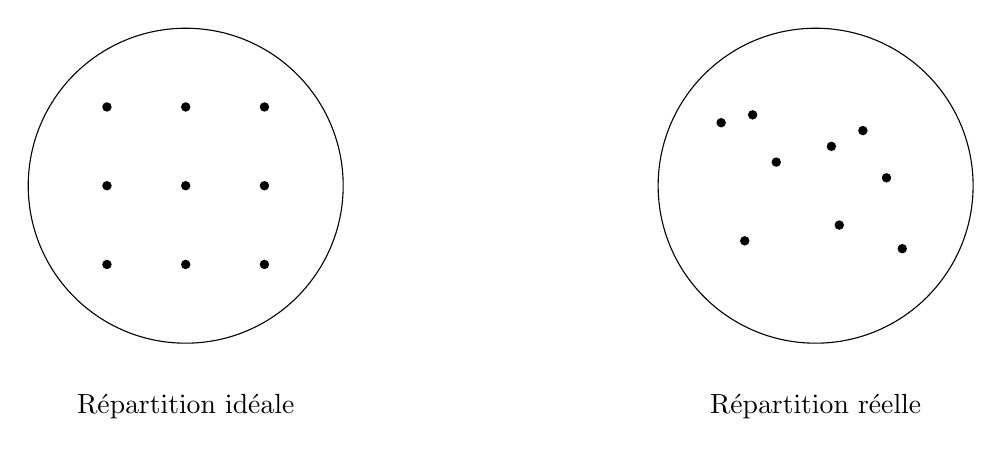
\begin{tikzpicture}

% Idéale
\draw (0,0) circle (2);

\foreach \x in {-1,0,1}
{
    \foreach \y in {-1,0,1}
    {
        \fill (\x,\y) circle (0.06);
    }
}

\node at (0,-2.8)
{Répartition idéale};

% Réelle
\begin{scope}[xshift=8cm]

\draw (0,0) circle (2);

\foreach \x/\y in {
-1.2/0.8,-0.8/0.9,-0.5/0.3,
0.2/0.5,0.6/0.7,
0.9/0.1,
-0.9/-0.7,
0.3/-0.5,
1.1/-0.8
}
{
\fill (\x,\y) circle (0.06);
}

\node at (0,-2.8)
{Répartition réelle};

\end{scope}

\end{tikzpicture}

\caption{Une gerbe réelle présente toujours des irrégularités.}
\label{fig:repartition_gerbe}

\end{figure}

\section{Le centre de la gerbe}

La densité d'impacts est souvent plus importante dans la partie centrale.

Cette concentration dépend notamment :

\begin{itemize}
    \item du choke ;
    \item de la cartouche ;
    \item du canon.
\end{itemize}

\section{Les trous dans la gerbe}

Certaines gerbes présentent des zones comportant peu ou pas d'impacts.

Ces zones sont souvent appelées :

\begin{quote}
trous
\end{quote}

Elles peuvent réduire l'efficacité pratique du tir.

\section{Influence de la bourre}

La conception de la bourre influence fortement :

\begin{itemize}
    \item la dispersion ;
    \item la régularité ;
    \item la densité centrale.
\end{itemize}

\section{Influence du choke}

Le choke modifie principalement :

\begin{itemize}
    \item le diamètre de la gerbe ;
    \item la densité des impacts ;
    \item la portée utile.
\end{itemize}

\begin{figure}[htbp]
\centering

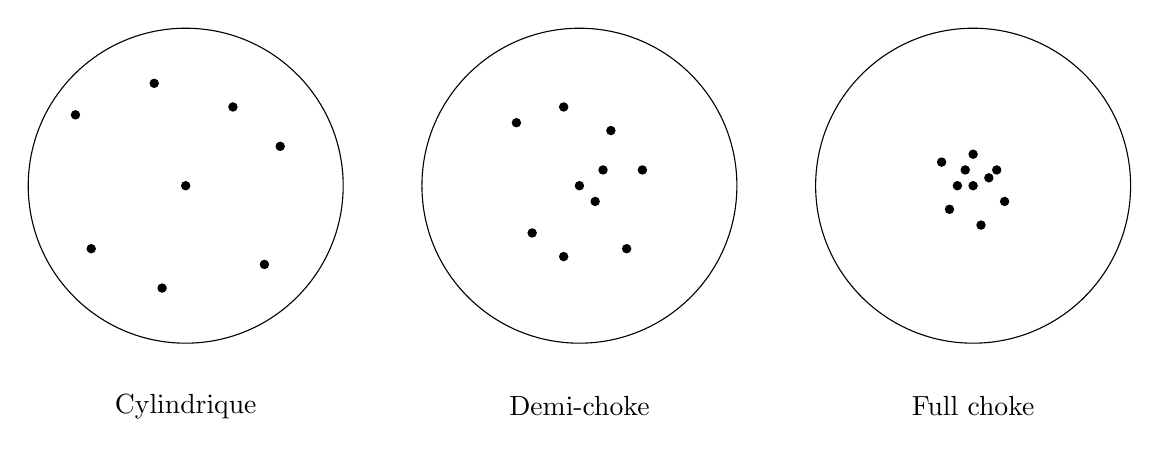
\begin{tikzpicture}

% Cylindrique
\draw (0,0) circle (2);

\foreach \x/\y in {
-1.4/0.9,-1.2/-0.8,
-0.4/1.3,0.6/1.0,
1.2/0.5,1.0/-1.0,
0.0/0.0,-0.3/-1.3
}
{
\fill (\x,\y) circle (0.06);
}

\node at (0,-2.8)
{Cylindrique};

% Demi
\begin{scope}[xshift=5cm]

\draw (0,0) circle (2);

\foreach \x/\y in {
-0.8/0.8,-0.6/-0.6,
-0.2/1.0,0.4/0.7,
0.8/0.2,0.6/-0.8,
0.0/0.0,-0.2/-0.9,
0.3/0.2,0.2/-0.2
}
{
\fill (\x,\y) circle (0.06);
}

\node at (0,-2.8)
{Demi-choke};

\end{scope}

% Full
\begin{scope}[xshift=10cm]

\draw (0,0) circle (2);

\foreach \x/\y in {
-0.4/0.3,-0.3/-0.3,
0.0/0.4,0.3/0.2,
0.4/-0.2,0.1/-0.5,
-0.2/0.0,0.0/0.0,
0.2/0.1,-0.1/0.2
}
{
\fill (\x,\y) circle (0.06);
}

\node at (0,-2.8)
{Full choke};

\end{scope}

\end{tikzpicture}

\caption{Illustration simplifiée de l'influence du choke sur la densité de la gerbe.}
\label{fig:choke_gerbe}

\end{figure}

\section{Influence de la grenaille}

Le diamètre et la masse des projectiles influencent également le comportement
de la gerbe.

Les résultats observés peuvent varier sensiblement selon les chargements.

\section{Essais sur cible}

Les performances d'une cartouche sont généralement évaluées par des tirs sur
cible.

Cette méthode permet de visualiser directement la gerbe obtenue.

\section{Cercles d'analyse}

Pour comparer les résultats, il est courant d'utiliser des cercles de diamètre
normalisé.

Les impacts contenus dans ces zones sont alors comptabilisés.

\begin{figure}[htbp]
\centering

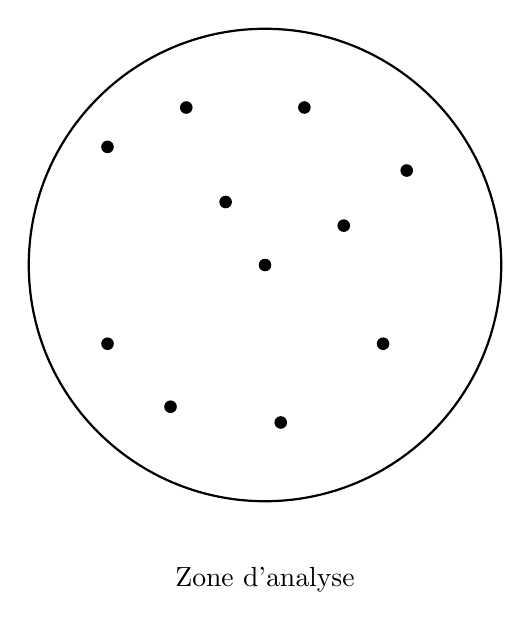
\begin{tikzpicture}

\draw[thick] (0,0) circle (3);

\foreach \x/\y in {
-2/1.5,-1/2,0.5/2,
1.8/1.2,
-2/-1,-1.2/-1.8,
0.2/-2,
1.5/-1,
0/0,
1/0.5,
-0.5/0.8
}
{
\fill (\x,\y) circle (0.08);
}

\node at (0,-4)
{Zone d'analyse};

\end{tikzpicture}

\caption{Exemple de cercle utilisé pour l'évaluation d'une gerbe.}
\label{fig:cercle_analyse}

\end{figure}

\section{Pourcentage de couverture}

Une mesure couramment utilisée consiste à calculer la proportion de projectiles
présents dans la zone étudiée.

Cette valeur permet de comparer différentes combinaisons :

\begin{itemize}
    \item cartouche ;
    \item choke ;
    \item canon.
\end{itemize}

\section{Pourquoi tester son arme ?}

Deux fusils apparemment identiques peuvent produire des gerbes différentes.

Les essais pratiques restent donc indispensables.

\section{Limites des valeurs théoriques}

Les recommandations générales fournissent des indications utiles.

Elles ne remplacent toutefois pas les observations réalisées avec l'arme
réellement utilisée.

\section{Vers les calibres de chasse}

La qualité d'une gerbe dépend de nombreux paramètres.

Avant d'examiner plus en détail les chargements, il convient de s'intéresser à
la notion de calibre dans les fusils de chasse.

\section{À retenir}

\begin{aretenir}

\begin{itemize}
    \item La gerbe résulte de la dispersion progressive de la grenaille.
    \item La densité des impacts est un paramètre essentiel.
    \item Les bourres et les chokes influencent fortement le résultat.
    \item Les essais sur cible constituent la méthode de référence.
    \item Les valeurs théoriques doivent être confirmées par l'expérience.
\end{itemize}

\end{aretenir}
